\documentclass{article}

% if you need to pass options to natbib, use, e.g.:
%     \PassOptionsToPackage{numbers, compress}{natbib}
% before loading neurips_2024

% ready for submission
\usepackage[preprint]{neurips_2024}


% to compile a preprint version, e.g., for submission to arXiv, add add the
% [preprint] option:
%     \usepackage[preprint]{neurips_2024}


% to compile a camera-ready version, add the [final] option, e.g.:
%     \usepackage[final]{neurips_2024}


% to avoid loading the natbib package, add option nonatbib:
%    \usepackage[nonatbib]{neurips_2024}


\usepackage[utf8]{inputenc} % allow utf-8 input
\usepackage[T1]{fontenc}    % use 8-bit T1 fonts
\usepackage{hyperref}       % hyperlinks
\usepackage{url}            % simple URL typesetting
\usepackage{booktabs}       % professional-quality tables
\usepackage{amsfonts}       % blackboard math symbols
\usepackage{nicefrac}       % compact symbols for 1/2, etc.
\usepackage{microtype}      % microtypography
\usepackage{xcolor}         % colors
\usepackage{array}
\usepackage{adjustbox}
\usepackage{amsmath}
\usepackage{float}
\usepackage{caption}
\usepackage{graphicx}
\usepackage{float} 
\usepackage{subfigure}
\usepackage{subcaption}
\usepackage{algorithm}
\usepackage{algpseudocode}
\usepackage{tikz}
\usepackage[utf8]{inputenc}
\usepackage{geometry}
\geometry{a4paper, margin=1in}

\usepackage{multirow} % 提供 \multirow 功能
\usepackage{makecell} % 支持 \makecell 功能

\hypersetup{
colorlinks=true,
linkcolor=blue,
filecolor=magenta,
urlcolor=cyan,
pdftitle={Example Title},
pdfpagemode=FullScreen,
}

\title{Numerical Optimization Project:\\ Analyzing ADMM and IRWA for Quadratic Programming}


% The \author macro works with any number of authors. There are two commands
% used to separate the names and addresses of multiple authors: \And and \AND.
%
% Using \And between authors leaves it to LaTeX to determine where to break the
% lines. Using \AND forces a line break at that point. So, if LaTeX puts 3 of 4
% authors names on the first line, and the last on the second line, try using
% \AND instead of \And before the third author name.


\author{%
  Hu Xinyue \And
  Zhuang Sihan \And
  Gao Shenghan
  % examples of more authors
  % \And
  % Coauthor \\
  % Affiliation \\
  % Address \\
  % \texttt{email} \\
  % \AND
  % Coauthor \\
  % Affiliation \\
  % Address \\
  % \texttt{email} \\
  % \And
  % Coauthor \\
  % Affiliation \\
  % Address \\
  % \texttt{email} \\
  % \And
  % Coauthor \\
  % Affiliation \\
  % Address \\
  % \texttt{email} \\
}


\begin{document}


\maketitle


\begin{abstract}
Quadratic Programming (QP) serves as a fundamental optimization problem in various domains, including finance, machine learning, and engineering. This paper investigates two QP solution methodologies: the Iterative Reweighted Algorithm (IRWA) and the Alternating Direction Method of Multipliers (ADMM). We address key challenges in these algorithms, including ill-conditioning, inconsistent penalty rates, and scaling issues, by incorporating \(\epsilon^{-1}\)-Threshold and scaling techniques. Extensive evaluations on generated QP instances reveal the complementary strengths of IRWA and ADMM, with IRWA demonstrating robustness in complex scenarios and ADMM excelling in computational efficiency. Our results underscore the importance of penalty synchronization and numerical stability in improving convergence rates and solution accuracy. The proposed enhancements make these methods more effective for a wide range of QP applications, bridging the gap between theory and real-world problem-solving.
\end{abstract}
\section{Introduction}
\subsection{Background}

\subsubsection{The Importance of Optimization Problems}
Optimization problems are integral to scientific and engineering fields, underpinning solutions in machine learning, economic modeling, and industrial design. These problems often translate real-world challenges into mathematical formulations, enabling data-driven decision-making and system optimization.

Quadratic Programming (QP), a fundamental optimization class, features a quadratic objective function and linear constraints, making it versatile and widely applicable. Key applications include:
\begin{itemize}
    \item \textup{Finance:} Portfolio optimization minimizes risks under budget constraints to determine optimal investments.
    \item \textup{Machine Learning:} Support Vector Machines (SVMs) use QP to maximize classification margins.
    \item \textup{Engineering:} Resource scheduling and path planning often rely on QP for objective modeling.
\end{itemize}

These use cases underscore the practical and theoretical importance of QP in optimization research.

\subsubsection{Mathematical Characteristics of Quadratic Programming}
A standard QP formulation is:
\[
\min_x \phi(x) = g^\top x + \frac{1}{2}x^{\top} H x \quad \textup{s.t.} A x + b \in C
\]
where:
\begin{itemize}
    \item $x \in \mathbb{R}^n$: decision variable.
    \item $g \in \mathbb{R}^n$: linear term coefficients.
    \item $H \in \mathbb{R}^{n \times n}$: symmetric quadratic term matrix.
    \item $A \in \mathbb{R}^{m \times n}$, $b \in \mathbb{R}^m$: constraint coefficients.
    \item $C$: feasible region (equality and inequality constraints).
\end{itemize}

\textbf{Convex vs. Non-Convex Problems:}
\begin{itemize}
    \item \textbf{Convex:} Positive semi-definite $H$ ensures global solutions and efficient algorithms.
    \item \textbf{Non-Convex:} Negative eigenvalues in $H$ introduce local minima, complicating global optimization.
\end{itemize}

This structure defines QP's theoretical challenges and its broad practical relevance.

\subsection{Research Objectives}

This project aims to explore Quadratic Programming by implementing and evaluating two optimization algorithms: Iterative Reweighting Algorithm (IRWA) and Alternating Direction Augmented Lagrangian (ADAL). The focus lies on their design, analysis, and performance in solving QP problems.

\subsubsection{Literature Review}
The initial phase involves a comprehensive review of existing QP methodologies. By examining state-of-the-art solvers, their benchmarks, and relevant theoretical insights, this research seeks to identify effective approaches and uncover potential areas for improvement. This review will inform the design and implementation of new or modified algorithms.


\subsubsection{Algorithm Implementation}
The implementation involves translating the theoretical principles of IRWA and ADAL into practical algorithms:
\begin{itemize}
    \item \textbf{IRWA:} Focuses on iterative reAnement by reweighting penalty terms to approximate the solution of exact penalty subproblems.
    \item \textbf{ADAL:} Utilizes an augmented Lagrangian framework to decouple constraints, solving subproblems in alternating directions while updatingmultipliers for constraint satisfaction.
\end{itemize}

\subsubsection{Core Objectives}
The core objectives are:
\begin{itemize}
    \item \textbf{Algorithm Implementation:} 
    \begin{itemize}
        \item Translate the theoretical principles of IRWA and ADAL into practical algorithms.
        \item Explore their behavior under various conditions, including convex, non-convex, and infeasible cases.
    \end{itemize}
    \item \textbf{Performance Analysis:} The project evaluates the algorithms on success rate, convergence rate, tolerance handling, scalability and solution quality.
\end{itemize}

% \subsubsection{Extended Objectives}
% Beyond standard QP scenarios, this project also investigates:
% \begin{itemize}
%     \item \textbf{Infeasibility Handling:} Strategies to address constraint conflicts.
%     \item \textbf{Non-Convex Problems:} Methods for solving non-convex QP without eigenvalue decompositions.
%     \item \textbf{Degenerate Cases:} Algorithm performance in singular or ill-defined solution spaces.
%     \item \textbf{Parameter Sensitivity:} Analysis of performance variation with parameter changes.
%     \item \textbf{Broader Applications:} Extensions to real-world problems beyond traditional QP.
% \end{itemize}

By addressing these goals, this project seeks to contribute to the advancement of robust and versatile QP solvers capable of meeting diverse computational demands.

\subsection{Structure of the Report}

This report outlines the objectives, methodology, and findings of the project. The structure is as follows:
\begin{itemize}
    \item \textbf{Introduction:} Background and objectives of QP research, including its mathematical foundation.
    \item \textbf{Literature Review:} Summary of existing QP solvers, their characteristics, strengths, and limitations.
    \item \textbf{Algorithm Implementation:} Details on IRWA and ADAL, including their mathematical formulations and implementation steps.
\item \textbf{Test, Evaluation, and Discussion:} Experimental setup, results on various QP instances, along with analysis, algorithm comparison, and potential improvements.
    \item \textbf{Conclusion:} Key findings and broader implications for QP research.
    \item \textbf{Reference}
    \item \textbf{Appendix}
\end{itemize}

\section{Review of Quadratic Programming Solvers}
Quadratic programming (QP) solvers are computational tools used to optimize quadratic objective functions subject to linear constraints. These solvers have broad applications in fields like finance, machine learning, control systems, and engineering. Modern QP solvers focus on achieving efficiency, robustness, scalability, and versatility. Iterative algorithms such as interior-point methods, active-set methods, and augmented Lagrangian techniques are central to these solvers.

\subsection{Quadratic Programming Solver Methods}

\subsubsection{Interior-Point Methods}
Interior-point methods are widely used for solving QP problems due to their efficiency and scalability. These methods solve the primal-dual KKT (Karush-Kuhn-Tucker) conditions iteratively by transforming the inequality constraints into logarithmic barrier terms:
\[
\min_{\mathbf{x}} \quad g^\top \mathbf{x} + \frac{1}{2} \mathbf{x}^\top H \mathbf{x} - \mu \sum_{i=1}^{m} \log(b - A \mathbf{x}),
\]
where $\mu > 0$ is the barrier parameter. As $\mu$ approaches zero, the solution converges to the optimal point.

The main advantages of interior-point methods are:
\begin{itemize}
    \item Efficient handling of large-scale QP problems with many constraints.
    \item Strong theoretical convergence guarantees for convex problems.
\end{itemize}
However, they require solving large linear systems at each iteration, which can be computationally expensive.

\subsubsection{Active-Set Methods}
Active-set methods iteratively adjust the set of active constraints, solving a sequence of equality-constrained subproblems. At each step, the algorithm identifies whether a constraint should be added to or removed from the active set based on the KKT conditions.

This approach is particularly useful for:
\begin{itemize}
    \item Problems with a small number of constraints relative to the problem size.
    \item Situations where the active set changes infrequently, leading to fewer iterations.
\end{itemize}

\subsubsection{First-Order Methods: Alternating Direction Method of Multipliers (ADMM)}
First-order methods are a class of algorithms used for solving optimization problems with a focus on efficiency and scalability. The Alternating Direction Method of Multipliers (ADMM) is one such method, well-suited for distributed optimization. ADMM decomposes the original problem into smaller subproblems that can be solved more efficiently in parallel.

For quadratic programming (QP) problems, ADMM splits the optimization variables $\mathbf{x}$ and reformulates the problem as:
\begin{align*}
\min_{\mathbf{x}, \mathbf{z}} &\quad g^\top \mathbf{x} + \frac{1}{2} \mathbf{x}^\top H \mathbf{x} \\
\text{s.t.} &\quad \mathbf{x} = \mathbf{z}, \quad A \mathbf{z} \leq \mathbf{b}.
\end{align*}
The method alternates between minimizing $\mathbf{x}$ and $\mathbf{z}$ while updating the Lagrange multipliers to enforce the constraints. The primary benefits of ADMM include:
\begin{itemize}
    \item Scalability for problems with separable structures, enabling the decomposition of complex problems into simpler subproblems.
    \item Parallelization potential, which makes ADMM suitable for large-scale or distributed systems, where each subproblem can be solved independently.
\end{itemize}
ADMM is particularly useful in applications involving sparse data, large datasets, and when the problem structure allows decomposition into smaller, easier-to-solve subproblems.


\subsubsection{Comparison of QP Solvers}
Each solver has distinct strengths and weaknesses, as summarized in Table~\ref{tab:qp-solver-comparison}. Interior-point methods are robust for dense problems, while active-set methods excel in sparsity scenarios. ADMM provides flexibility in distributed settings but may require careful parameter tuning.


\begin{table}[h]
\centering
\caption{Comparison of QP Solvers}
\label{tab:qp-solver-comparison}
\begin{adjustbox}{max width=\textwidth}
\begin{tabular}{|l|l|l|}
\hline
\textbf{Method}            & \textbf{Advantages}                                  & \textbf{Disadvantages} \\ \hline
Interior-Point             & Robust, scalable, strong convergence guarantees      & High computational cost for dense problems \\ \hline
Active-Set                 & Efficient for sparse or small-scale problems          & May be slow for problems with many constraints \\ \hline
ADMM                       & Scalable, suitable for distributed optimization       & Requires parameter tuning, slow convergence \\ \hline
\end{tabular}
\end{adjustbox}
\end{table}

\subsection{Modern QP Solvers}

\subsubsection{Evolution of Quadratic Programming Solvers}


\begin{center}
\begin{tikzpicture}[line width=0.5pt, every node/.style={font=\small}, x=0.75cm, y=1cm]

% Draw timeline vertical line
\draw[thick] (0, 0) -- (0, 14);

% Add year markers and connecting lines
\foreach \y in {13.5, 12.5, 11.5, 10.5, 9.5, 8.5, 7.5, 6.5, 5.5, 4.5, 3.5, 2.5, 1.5, 0.5} {
    \draw[-] (0, \y) -- (0.5, \y); % Horizontal connection
}

% Add events on the timeline
\node[anchor=west] at (0.5, 13.5) {The Goldfarb-Idnani (quadprog) is introduced.};
\node[anchor=west] at (0.5, 12.5) {QPOASES is developed at Freiburg University.};
\node[anchor=west] at (0.5, 11.5) {MOSEK (Denmark) is released.};
\node[anchor=west] at (0.5, 10.5) {\href{https://www.seas.ucla.edu/~vandenbe/publications/coneprog.pdf}{CVXOPT} is launched by Eindhoven University of Technology.};
\node[anchor=west] at (0.5, 9.5) {Gurobi Optimization Inc. releases Gurobi solver.};
\node[anchor=west] at (0.5, 8.5) {ECOS (Boyd Team, Stanford) becomes available.};
\node[anchor=west] at (0.5, 7.5) {OSQP is introduced by Imperial College London.};
\node[anchor=west] at (0.5, 6.5) {\href{https://doi.org/10.1109/LRA.2019.2926664}{qpSWIFT} is developed by Aydin Idil.};
\node[anchor=west] at (0.5, 5.5) {HiGHS solver is developed at the University of Leeds.};
\node[anchor=west] at (0.5, 4.5) {DAQP is launched by ETH Zurich.};
\node[anchor=west] at (0.5, 3.5) {PIQP by Tobias Koch Team is released.};
\node[anchor=west] at (0.5, 2.5) {Clarabel (Boyd Team) becomes available.};
\node[anchor=west] at (0.5, 1.5) {\href{https://hal.inria.fr/hal-03683733/file/Yet_another_QP_solver_for_robotics_and_beyond.pdf/}{ProxQP} is launched by Inria and ENS Paris Team.};
\node[anchor=west] at (0.5, 0.5) {SCS and HPIPM are introduced.};

% Add year labels to the left of the timeline
\node[anchor=east] at (-0.2, 13.5) {1983};
\node[anchor=east] at (-0.2, 12.5) {1990s};
\node[anchor=east] at (-0.2, 11.5) {2000};
\node[anchor=east] at (-0.2, 10.5) {2013};
\node[anchor=east] at (-0.2, 9.5) {2013};
\node[anchor=east] at (-0.2, 8.5) {2014};
\node[anchor=east] at (-0.2, 7.5) {2016};
\node[anchor=east] at (-0.2, 6.5) {2017};
\node[anchor=east] at (-0.2, 5.5) {2018};
\node[anchor=east] at (-0.2, 4.5) {2019};
\node[anchor=east] at (-0.2, 3.5) {2020};
\node[anchor=east] at (-0.2, 2.5) {2021};
\node[anchor=east] at (-0.2, 1.5) {2021};
\node[anchor=east] at (-0.2, 0.5) {2022};

\end{tikzpicture}
\end{center}

The timeline of QP solver development, as illustrated in figure~\ref{fig:timeline}, highlights the progression of solver technologies over the decades. 

\begin{figure}[ht]
\centering
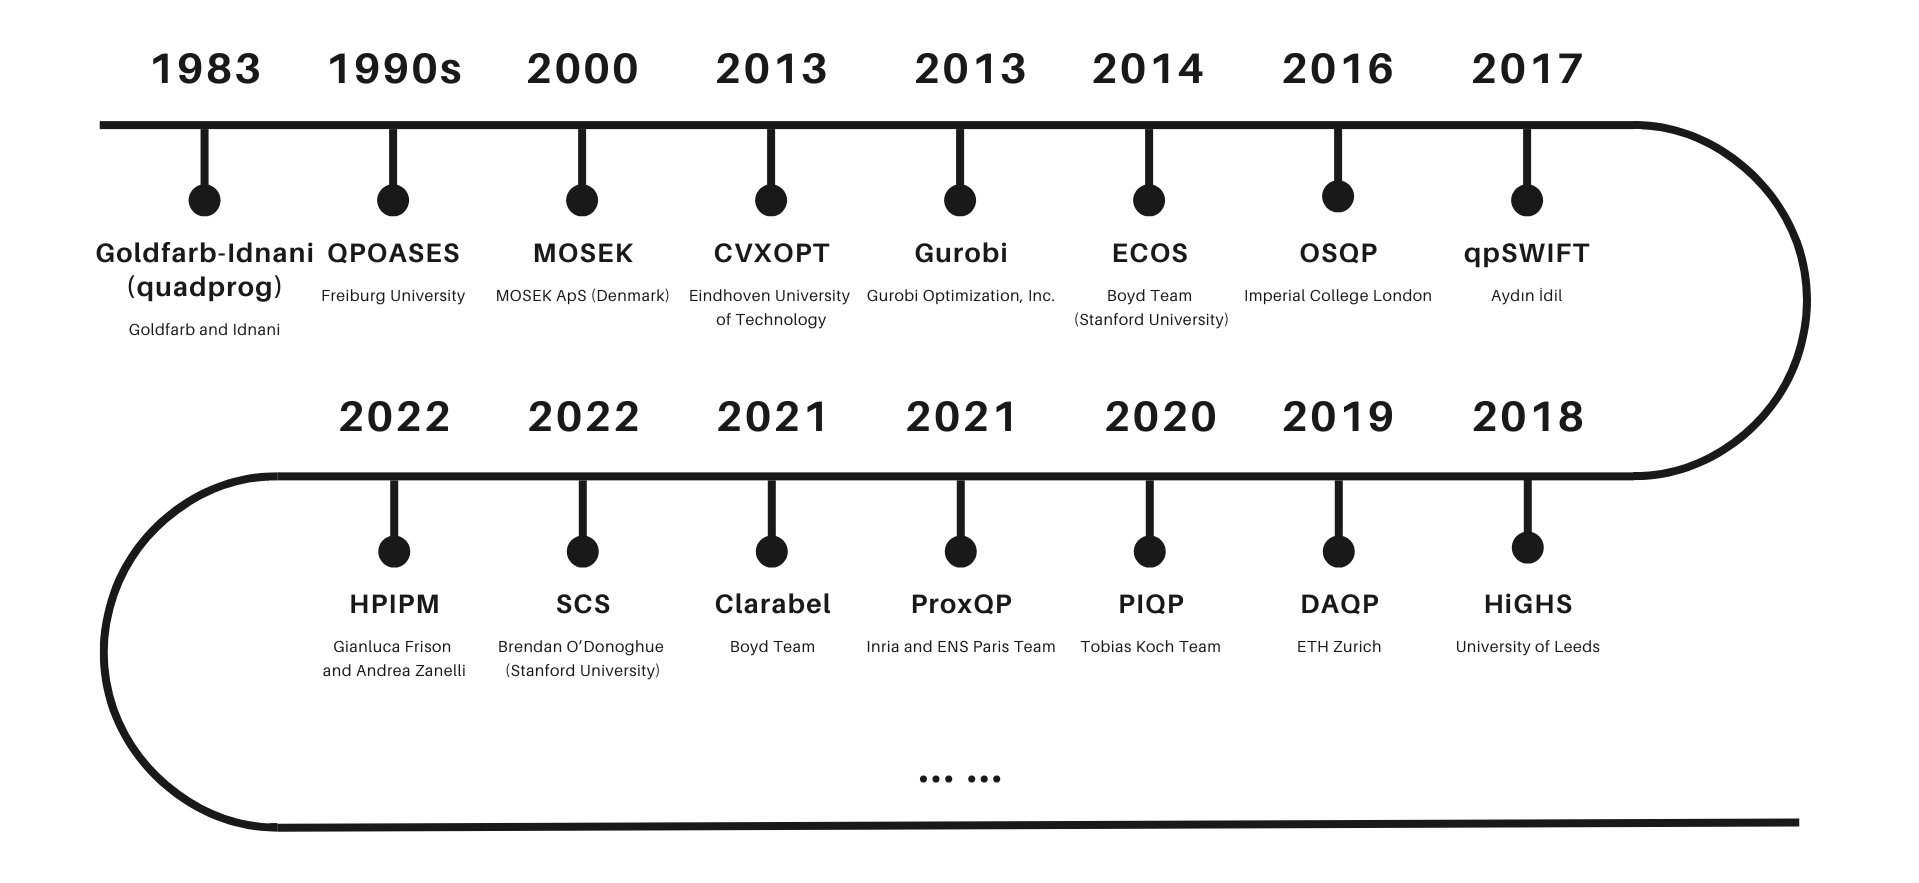
\includegraphics[width=0.77\textwidth]{fig/timeline.jpg}
\caption{Timeline of QP Solvers Development}
\label{fig:timeline}
\end{figure}

These trends underline the dynamic evolution of QP solvers, catering to diverse optimization challenges across commercial, academic, and embedded contexts: 

\begin{itemize}
    \item \textup{Commercial Solvers:} Early solvers such as Gurobi and MOSEK emerged in the late 20th and early 21st centuries, offering robust solutions for industrial-scale optimization.
    \item \textup{Open-Source Solvers:} The rise of open-source solvers, including OSQP, HiGHS, and SCS, began after 2010, driven by the need for academic transparency and meeting industrial requirements.
    \item \textup{Embedded and Real-Time Optimization:} Recent years have witnessed a surge in solvers like DAQP and HPIPM, designed specifically for embedded systems and real-time applications.
\end{itemize}

\subsubsection{Classification and Solver Characteristics}
QP solvers are categorized based on their supported problem types, scale, and underlying algorithms:
\begin{itemize}
    \item \textbf{Problem Types:} 
    \begin{itemize}
        \item Most solvers (e.g., OSQP, ECOS) target convex problems, ensuring global solutions.
        \item Solvers like Gurobi and CPLEX handle non-convex cases, often at higher computational costs.
    \end{itemize}
    \item \textbf{Problem Scale:}
    \begin{itemize}
        \item Small-scale problems are addressed efficiently by solvers such as QPOASES.
        \item Large-scale sparse problems are handled by HiGHS and Gurobi, optimized for industrial-grade applications.
    \end{itemize}
    \item \textbf{Algorithmic Types:}
    \begin{itemize}
        \item \textbf{Interior-Point Methods:} Focus on high-precision optimization (e.g., CVXOPT, MOSEK).
        \item \textbf{Active-Set Methods:} Excel in solving dense, small-scale problems (e.g., QPOASES).
        \item \textbf{Augmented Lagrangian Methods:} Balance dense and sparse problem handling (e.g., ProxQP).
        \item \textbf{Other Methods:} Leverage specialized techniques like Douglas–Rachford splitting for sparse matrices (e.g., OSQP).
    \end{itemize}
\end{itemize}

\subsubsection{Key Solvers and Their Applications}
The following table~\ref{tab:solver-characteristics} summarizes key QP solvers and their applications:
\begin{table}[ht]
\centering
\caption{Characteristics of Major QP Solvers}
\begin{adjustbox}{max width=\textwidth}
\begin{tabular}{|l|l|l|l|l|}
\hline
\textbf{Solver} & \textbf{Algorithm Type}      & \textbf{Supported Problem Type} & \textbf{Matrix Features} & \textbf{Application Scenarios}     \\ \hline
OSQP            & Douglas–Rachford            & Convex Problems                 & Sparse                   & Embedded systems, real-time control \\ \hline
Gurobi          & Interior Point + Mixed Integer & Convex and Non-Convex Problems  & Sparse                   & Financial optimization, engineering \\ \hline
HiGHS           & Active Set                  & Convex Problems                 & Sparse                   & Industrial-scale optimization       \\ \hline
ProxQP          & Augmented Lagrangian        & Convex Problems                 & Dense and Sparse         & High-precision optimization         \\ \hline
CVXOPT          & Interior Point              & Convex Problems                 & Dense                    & Academic research, simulations      \\ \hline
QPOASES         & Active Set                  & Convex Problems                 & Dense                    & Small-scale real-time optimization  \\ \hline
MOSEK           & Interior Point              & Convex Problems                 & Sparse                   & High-precision financial optimization \\ \hline
Clarabel        & Interior Point              & Convex Problems                 & Sparse                   & Control, Optimization in Sparse Systems \\ \hline
DAQP            & Active Set                  & Convex Problems                 & Dense                    & Real-time Optimization, Robotics     \\ \hline
ECOS            & Interior Point              & Convex Problems                 & Sparse                   & Financial Optimization, Control      \\ \hline
HPIPM           & Interior Point              & Convex Problems                 & Dense                    & Embedded Optimization, MPC           \\ \hline
PIQP            & Proximal Interior Point     & Convex Problems                 & Dense and Sparse         & Quadratic Programming, Portfolio Optimization \\ \hline
qpSWIFT         & Interior Point              & Convex Problems                 & Sparse                   & Small-scale optimization, research   \\ \hline
quadprog        & Goldfarb-Idnani             & Convex Problems                 & Dense                    & Academic research, prototyping       \\ \hline
SCS             & Douglas–Rachford            & Convex Problems                 & Sparse                   & Large-scale optimization, control    \\ \hline
\end{tabular}
\end{adjustbox}
\label{tab:solver-characteristics}
\end{table}

\subsection{Performance and Benchmarks}

\subsubsection{Performance Metrics}
Evaluating QP solvers involves metrics such as:
\begin{itemize}
    \item \textbf{Success Rate}: Proportion of solved problems, reflecting robustness.
    \item \textbf{Runtime Efficiency}: Solution time, critical for real-time/large-scale use.
    \item \textbf{Stability}: Ability to converge reliably under varying conditions, such as ill-conditioned problems or different numerical tolerances, measured through:

    \begin{itemize}
        \item \textup{Primal Residual}: Maximum error on equality and inequality constraints at the returned solution.
        \item \textup{Dual Residual}: Maximum error on the dual feasibility condition at the returned solution.
        \item \textup{Duality Gap}: Measure of the gap between primal and dual solutions.
    \end{itemize}
\end{itemize}

\subsubsection{Performance Comparison Based on Benchmarks}
The Maros-Meszaros dataset benchmarks solver performance across 138 problems, including:
\begin{itemize}
    \item Dense problems (62 instances): Test computational efficiency with small, dense matrices.
    \item Sparse problems: Assess scalability for large-scale scenarios.
\end{itemize}

Figure~\ref{fig:solver-performance} shows solver performance on the dense subset with high accuracy. The x-axis represents runtime (log scale), and the y-axis indicates the number of problems solved.

\begin{figure}[ht]
\centering
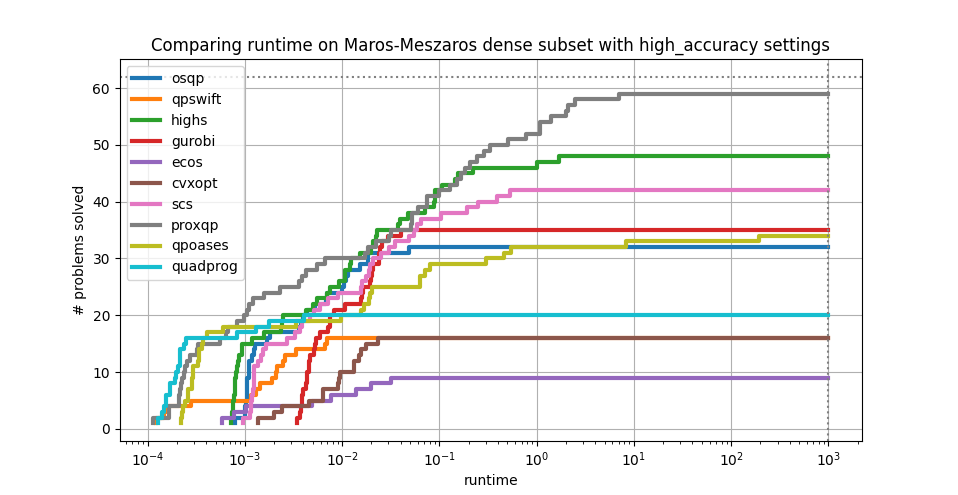
\includegraphics[width=\textwidth]{fig/runtimegraph.png}
\caption{Solver performance on Maros-Meszaros dense subset under high-accuracy settings}
\label{fig:solver-performance}
\end{figure}

\subsubsection{Comprehensive Performance Analysis}
The Table~\ref{tab:benchmark-performance} below shows the performance comparison of different QP solvers based on Benchmark tests:
\begin{table}[ht]
\centering
\caption{Performance Comparison of Solvers Based on Benchmark Tests}
\begin{adjustbox}{max width=\textwidth}
\begin{tabular}{|l|l|l|l|}
\hline
\textbf{Solver}    & \textbf{Success Rate}          & \textbf{Computation Time}           & \textbf{Stability Metrics}                     \\ \hline
OSQP               & High for convex problems       & Fast for sparse problems            & Stable primal and dual residuals               \\ \hline
Gurobi             & Very high (convex + nonconvex) & Fast with multithreaded support     & Robust across all metrics                      \\ \hline
HiGHS              & Moderate                      & Fast for sparse problems            & Reliable for large-scale convex problems       \\ \hline
ProxQP             & High for precision modes       & Moderate                            & Excellent numerical stability                  \\ \hline
CVXOPT             & High for small-medium size     & Slow                                & Stable for dense problems                      \\ \hline
\end{tabular}
\end{adjustbox}
\label{tab:benchmark-performance}
\end{table}

\begin{itemize}
    \item \textbf{Success Rate:} 
    \begin{itemize}
        \item Gurobi demonstrates nearly perfect success across problem types, excelling in both convex and non-convex cases.
        \item OSQP excels in sparse and convex scenarios, suitable for real-time applications.
        \item ProxQP performs well in high-accuracy modes but requires more runtime for complex problems.
    \end{itemize}
    \item \textbf{Runtime Efficiency:}
    \begin{itemize}
        \item OSQP and HiGHS are highly efficient for sparse problems, ideal for large-scale applications.
        \item Gurobi, with multithreaded support, achieves superior runtime across diverse problem sizes.
        \item ProxQP balances precision and runtime, particularly effective for dense problems.
    \end{itemize}
    \item \textbf{Stability and Scalability:}
    \begin{itemize}
        \item Gurobi and ProxQP maintain robust convergence under varying conditions.
        \item OSQP shows reliable performance in embedded systems requiring fast convergence.
        \item CVXOPT struggles with large-scale or highly complex problems.
    \end{itemize}
\end{itemize}



% \subsection{Challenges and Developments}

% \subsubsection{Challenges and Limitations}
% Despite advancements, key challenges persist:
% \begin{itemize}
% 	\item \textup{Non-Convex Problems}:
% Open-source solvers like OSQP and HiGHS struggle with non-convex problems, where global optimization remains a challenge.
% 	\item \textup{Large-Scale Instability}:
% Numerical instability arises in large-scale dense problems, with solvers like CVXOPT facing scalability issues.

% 	\item \textup{Parameter Sensitivity}:
% Solvers depend heavily on:
% \begin{itemize}
%     \item \textup{Initial Guesses}: Poor guesses lead to suboptimal results.
%     \item \textup{Tolerances}: Tight tolerances increase runtime; loose ones affect accuracy.
% \end{itemize}

% 	\item \textup{Nonlinear Constraints}:
% Support for nonlinear constraints is limited, restricting applications in engineering and physics.

%     \item \textup{Implementation Challenges}:
%     \begin{itemize}
%         \item Parallel processing efficiency
%         \item Memory management in large-scale problems
%     \end{itemize}

%     \item \textup{Theoretical Limitations}:
%     \begin{itemize}
%         \item NP-hardness of non-convex problems
%         \item Convergence guarantees often limited to convex cases
%         \item Gap between theoretical bounds and practical performance
%         \item Difficulty in proving global optimality
%     \end{itemize}
% \end{itemize}


% \subsubsection{Future Directions}
% Potential improvements include:
% \begin{itemize}
%     \item Efficient algorithms for non-convex problems.
%     \item Enhanced sparse matrix handling and parallel computing for scalability.
%     \item Robust parameter tuning for reliability.
%     \item Expanded support for nonlinear constraints.
% \end{itemize}

% Addressing these issues will enhance solver applicability and efficiency in diverse real-world scenarios.

\section{Algorithm Implementation}
\subsection{IRWA}
\subsubsection{Origin Algorithm}
The Iterative Reweighted Algorithm (IRWA) is a penalty-based optimization method designed to solve quadratic programming (QP) problems through the approximation of exact penalty subproblems. The algorithm iteratively minimizes a reweighted quadratic objective, updating weights and relaxation vectors dynamically to handle constraints effectively. IRWA is especially suited for problems where constraints are challenging to satisfy or infeasibility is a concern.

Key characteristics of IRWA include:
\begin{itemize}
    \item \textbf{Dynamic Weight Adjustment:} Iterative updates of weight vectors ensure constraint satisfaction while refining the solution.
    \item \textbf{Exact Penalty Approximation:} The use of reweighted penalties closely approximates the original constrained problem.
    \item \textbf{Scalability and Robustness:} Effective for handling high-dimensional and challenging QP problems.
\end{itemize}

\begin{algorithm}[H]
\caption{IRWA}
\label{alg:IRWA}
\begin{algorithmic}[1]
\Require Initial values $x^0$, $\epsilon^0 > 0$, parameters $\eta \in (0, 1)$, $\gamma > 0$, $M > 0$, $\text{tol}_{\text{prim}}$, $\text{tol}_{\text{dual}}$, and maximum iterations $k_{\text{max}}$
\State Initialize iteration counter $k = 0$
\Repeat
    \State 
    \begin{align}\label{ori-w-update}
    w_i(x, \epsilon) :&=
    \begin{cases}
    \big(|a_i^\top x + b_i|^2 + \epsilon_i^2\big)^{-1/2}, & i \in \mathcal{I}_1, \\
    \big(\max\{(a_i^\top x + b_i), 0\}^2 + \epsilon_i^2\big)^{-1/2}, & i \in \mathcal{I}_2,
    \end{cases}
    \end{align}
    \State $W_k = \text{diag}(w_i^k)$
    \State $x^{k+1} \gets \arg\min_x \, g^\top x + \frac{1}{2} x^\top H x + \frac{1}{2} (A x + b)^\top W_k (A x + b)$
    \State 
    $r_i^k = (1 - v_i^k)(A_i x^k + b_i)$
    \State
    $ q_i^k = A_i (x^{k+1} - x^k)$
    \If{$|q_i^k| \leq M \cdot \big((r_i^k)^2 + \epsilon_k^2\big)^{0.5+\gamma}$}
    \State $\quad \epsilon_i^{k+1} \gets \eta \cdot \epsilon_i^k$
    \EndIf
    \Until{termination criterion is satisfied}
%     \State
%     \[
%     \text{Terminate if } \|x^{k+1} - x^k\|_2 \leq \text{tol}_{\text{prim}} \text{ and } \|\epsilon^k\|_2 \leq \text{tol}_{\text{dual}}
%     \]
%     \State Update iteration counter $k \gets k + 1$
% \Until{Stopping criteria are met or $k \geq k_{\text{max}}$}
\end{algorithmic}
\end{algorithm}

\begin{figure}[H]
    \centering
    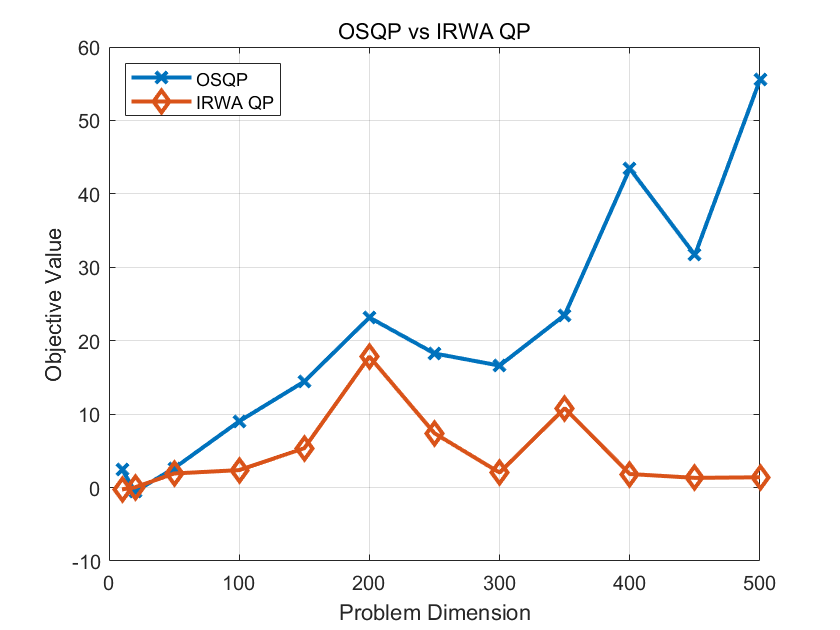
\includegraphics[width=0.75\linewidth]{fig/OSQP_vs_origin.png}
    \caption{OSQP vs origin IRWA}
    \label{fig:enter-label}
\end{figure}

This figure shows a comparison of the original IRWA algorithm and the OSQP optimal solution. The difference between IRWA and OSQPacross varying dimensions are highlighted. We can also find that optimal value are always lower than those of OSQP.

\subsubsection{IRWA with \(\mathbf{\epsilon^{-1}}\)-Threshold}
We observed that the rate at which equality and inequality constraints were penalized to reach the feasible domain was not consistent, which led to the original algorithm producing lower objective values than the OSQP solver. This inconsistency arises due to penalty weights not being on the same scale, which encourages the algorithm to violate equality constraints(which achieves the feasible domain slower and thus has much smaller penalty weights) to achieve a lower objective value. To handle this problem, we implemented the \({\epsilon^{-1}}\)-Threshold to ensure proper penalty synchronization.
% The \(\epsilon^{-1}\) threshold is crucial for achieving constant alignment, magnitude alignment, and synchronizing penalties within the feasible domain in the IRWA algorithm. It ensures numerical stability and balanced treatment of constraints during optimization.
\paragraph{Methodology}
\begin{itemize}
    \item \textbf{Alignment}: 
    The \(\epsilon^{-1}\)-threshold serves as a lower bound for the penalty weights and thus aligns the weights across equality and inequality constraints.
    
    The \(\epsilon^{-1}\)-threshold method is performed after computing \ref{ori-w-update} and the weight $w_i$ for each iteration is updated as:
    \begin{equation}
    w_i \leftarrow \max\left(w_i, \epsilon^{-1}\right)
    \end{equation}
    This ensures consistent penalty weighting scale between equality and inequality constraints.

    % \item \textbf{Magnitude Alignment}: 
    % By dynamically scaling weights, the threshold ensures constraints with larger residuals are penalized appropriately, avoiding over-penalization of smaller residuals.

    % \item \textbf{Synchronization with Feasible Domain}: 
    % The relaxation parameter \(\epsilon\) is iteratively updated as:
    % \[
    % \epsilon^{k+1} = \eta \cdot \epsilon^k, \quad \text{where } \eta \in (0, 1).
    % \]
    % This progressive adjustment ensures penalties remain aligned with the feasible region.
\end{itemize}



\begin{figure}[H]
    \centering
    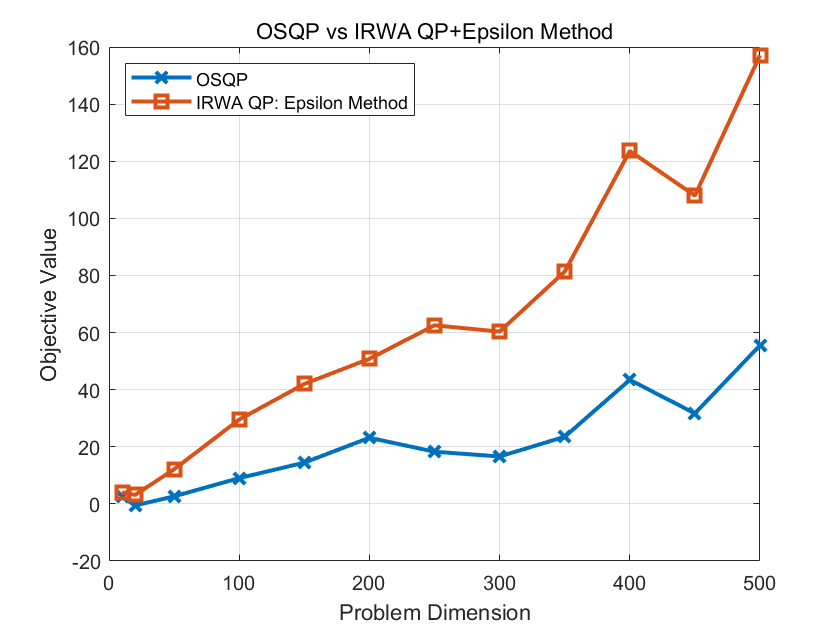
\includegraphics[width=0.75\linewidth]{fig/OSQP_vs_Epsilon_Method.png}
    \caption{OSQP vs IRWA+Epsilon Method}
    \label{fig: OSQP vs Epsilon Method}
\end{figure}


\subsubsection{IRWA with  \(\mathbf{\epsilon^{-1}}\)-Threshold and Scaling on}
We observed that when \(\epsilon\) drops quickly, (i.e. the penalty weights rises fast), the linear system becomes ill-conditioned and the algorithm terminated before reaching the optimal point. To address this, we performed a matrix scaling method.\cite{Stellato2020}

% Scaling plays a crucial role in improving numerical stability and convergence in the IRWA algorithm. It ensures that equality and inequality constraints are treated uniformly, especially when the constraints vary significantly in magnitude. In our implementation, scaling is applied to both the constraint matrix and the corresponding vector.

\paragraph{Methodology}
\begin{itemize}
    \item \textbf{Scaling Factors}: 
    The Frobenius norm of $A_1$ (equality constraint matrix) is used to compute the scaling factor for equality constraints, while the Frobenius norm of $A_2$ (inequality constraint matrix) is used for inequality constraints:
    \[
    \text{scale\_eq} = \frac{1}{\|A_1\|_F}, \quad \text{scale\_ineq} = \frac{1}{\|A_2\|_F}.
    \]

    \item \textbf{Scaling Matrix}: 
    A diagonal scaling matrix is constructed using the computed scaling factors:
    \[
    S = \text{diag}([\text{scale\_eq} \cdot \mathbf{1}_{m_{\text{eq}}}; \text{scale\_ineq} \cdot \mathbf{1}_{m_{\text{ineq}}}]),
    \]
    where $m_{\text{eq}}$ and $m_{\text{ineq}}$ are the number of equality and inequality constraints, respectively.

    \item \textbf{Transformation}:
    The constraint matrix $A$ and vector $b$ are scaled as:
    \[
    A_{\text{scaled}} = S \cdot A, \quad b_{\text{scaled}} = S \cdot b.
    \]
    Similarly, the weight vector $w$ and other associated terms are scaled within each iteration.
\end{itemize}

The scaling approach ensures:
\begin{enumerate}
    \item Improved Numerical Stability: The rescaled problem reduces sensitivity to \textbf{ill-conditioned} matrices, particularly in $A_1$ and $A_2$.
    \item Faster Convergence: The iterative solution benefits from a more balanced problem structure, leading to stable and efficient updates.
\end{enumerate}

% \noindent Figure~ compares the objective function values across different problem sizes. The results show the effectiveness of scaling, where ``Scale QP'' achieves values closer to ``Optimal'' compared to unscaled ``QP.''

% \subsubsection{IRWA with Scaling and \(\mathbf{\epsilon^{-1}}\)-Threshold}
Combining \(\mathbf{\epsilon^{-1}}\)-Threshold with Scaling, we obtain the final algorithm:
\begin{algorithm}[H]\label{scal-ep}
\caption{IRWA with Scaling and \(\epsilon^{-1}\)-Threshold}
\label{alg:IRWA_Scaling_Epsilon}
\begin{algorithmic}[1]
\Require Initial values $x^0$, $\epsilon^0 > 0$, parameters $\eta \in (0, 1)$, $\gamma > 0$, $M > 0$, $\text{tol}_{\text{prim}}$, $\text{tol}_{\text{dual}}$, and maximum iterations $k_{\text{max}}$, $A_1$, $A_2$ ,$b_1$, $b_2$, $g$,$H$
\State 
$
\text{scale\_eq} = \frac{1}{\|A_1\|_F}, \quad \text{scale\_ineq} = \frac{1}{\|A_2\|_F}
$
\State 
$S = \text{diag}([\text{scale\_eq} \cdot \mathbf{1}_{m_{\text{eq}}}; \text{scale\_ineq} \cdot \mathbf{1}_{m_{\text{ineq}}}])$

\State 
$A_{\text{scaled}} = S \cdot A, \quad b_{\text{scaled}} = S \cdot b$

\Repeat
\State
    \begin{align*}
    w_i(x, \epsilon) :&=
    \begin{cases}
    \big(|a_i^\top x + b_i|^2 + \epsilon_i^2\big)^{-1/2}, & i \in \mathcal{I}_1, \\
    \big(\max\{(a_i^\top x + b_i), 0\}^2 + \epsilon_i^2\big)^{-1/2}, & i \in \mathcal{I}_2,
    \end{cases}
    \end{align*}
    \State $w_i\leftarrow \max(w_i,\epsilon^{-1})$
    \State $W_k = \text{diag}(w_i^k)$
    \State 
    $
    x^{k+1} \gets \arg\min_x \, g^\top x + \frac{1}{2} x^\top H x + \frac{1}{2} (A_{\text{scaled}} x + b_{\text{scaled}})^\top W_k (A_{\text{scaled}} x + b_{\text{scaled}})
    $
    \State 
    $
    r_i^k = (1 - v_i^k)(A_{\text{scaled}, i} x^k + b_{\text{scaled}, i})$ 
    \State $q_i^k = A_{\text{scaled}, i} (x^{k+1} - x^k)
    $
    \If{
    $
    |q_i^k| \leq M \cdot \big((r_i^k)^2 + \epsilon_k^2\big)^{0.5+\gamma}, \, \forall i
    $
    }
        \State 
        $\epsilon_i^{k+1} \gets \eta \cdot \epsilon_i^k$
    \EndIf
    \Until{termination criterion is satisfied}
\end{algorithmic}
\end{algorithm}

\begin{figure}[H]
    \centering
    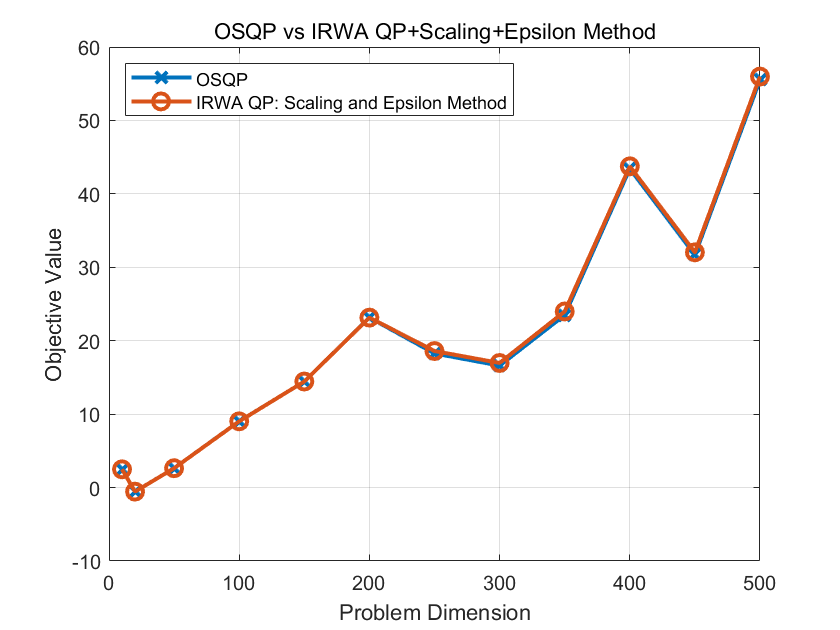
\includegraphics[width=0.75\linewidth]{fig/OSQP_vs_Scaling+Epsilon.png}
    \caption{OSQP vs IRWA+Scaling+Epsilon}
    \label{fig:OSQP vs IRWA+Scaling+Epsilon}
\end{figure}
Figure~\ref{fig:OSQP vs IRWA+Scaling+Epsilon} illustrates the comparison between OSQP and IRWA with the combined Scaling and \(\epsilon^{-1}\)-Threshold methods. 

\begin{itemize}
    \item The combined method achieves objective values almost identical to OSQP across all problem dimensions, indicating its effectiveness in maintaining optimality.

    \item The method demonstrates consistent performance, avoiding divergence or instability even for high-dimensional problems.

    \item  Using only \(\epsilon^{-1}\)-Threshold or Scaling independently leads to deviations from the OSQP baseline, the combined approach successfully balances penalty synchronization and numerical stability.
\end{itemize}

These results confirm that incorporating both Scaling and \(\epsilon^{-1}\)-Threshold into IRWA enhances its robustness and makes it highly competitive with state-of-the-art solvers like OSQP.

\subsubsection{Comparison Test}
\begin{figure}[H]
    \centering
    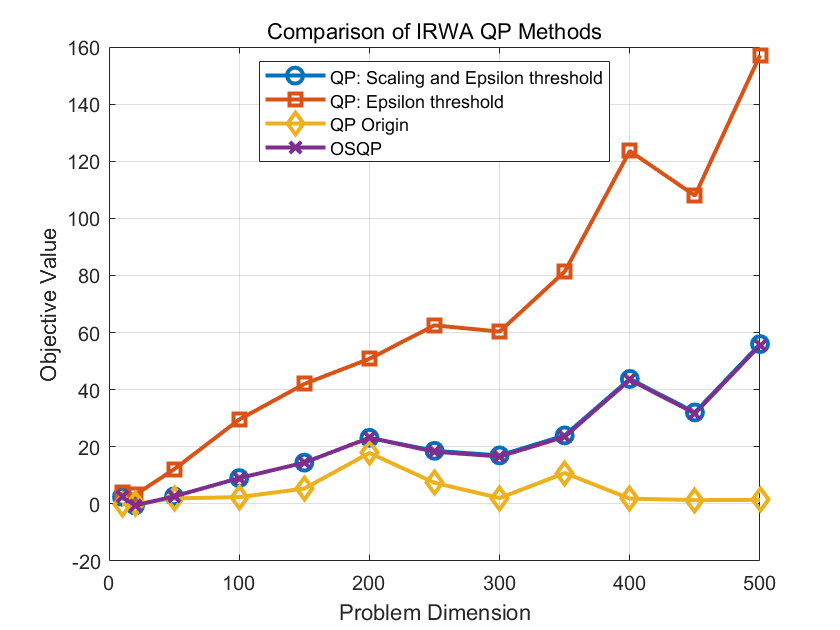
\includegraphics[width=0.75\linewidth]{fig/IRWA_Comparison_Conclude.png}
    \caption{Conclusion of IRWA QP and enhance methods}
    \label{fig:Conclusion of IRWA QP and enhance methods}
\end{figure}

The results in Figure~\ref{fig:Conclusion of IRWA QP and enhance methods} show that combining the \(\epsilon^{-1}\)-Threshold and Scaling methods significantly improves the IRWA algorithm:

1. The combined method achieves objective values nearly identical to those of OSQP across all dimensions, ensuring optimality and accuracy.

2. \(\epsilon^{-1}\)-Threshold alone results in higher objective values, while Scaling alone underestimates the optimal values. The combined approach effectively balances penalties for better performance.

3. The combined method remains robust and consistent as problem dimensions increase, avoiding divergence or instability.

This demonstrates that the combined \(\epsilon^{-1}\)-Threshold and scaling approach is reliable and comparable to OSQP, offering both stability and optimality for QP problems.

\subsection{ADMM}
\subsubsection{Origin Algorithm}
The Accelerated Distributed Augmented Lagrangian (ADAL) is a variant of the ADMM algorithm designed to address convergence issues in multi-block optimization problems under Jacobian decomposition\cite{yang2022surveyadmmvariantsdistributed}. ADAL introduces a correction step that modifies only the primal variables to ensure convergence in a broader set of scenarios.

Conjugate Gradient (CG) is used to solve the linear system in each iteration, making the method scalable to large problems.


% \begin{table*}[h]
% \setlength\tabcolsep{2pt}
% \renewcommand\arraystretch{1}
% \centering
% \caption{ADMM variants for solving multi-block problem}
% \label{tab:multi-block_ADMM}
% \begin{tabular}{llllll}   
% 	\hline 
% 	\textbf{Methods}  & \textbf{Main assumptions}  & \textbf{Types} & \textbf{Convergence}  & \textbf{Features}  \\
% 	\hline
% 	\multirow{4}{*}{\makecell[l]{~\\~\\~\\~\\~\\Classic ADMM}}   & \makecell[l]{$n-1$ $f_i$ strongly convex. \\ Existence of saddle points.} & Gauss-Seidel &  \makecell[l]{Global convergence. \\ Global optima. \\ Convergence rate $\mathcal{O}(1/k)$.}  & \makecell[l]{Arbitrary $n$ blocks. \\ Convex.} \\
% 	\cline{2-6}
% 	& \makecell[l]{$n = 3$. \\ $f_1$ strongly convex \\ or $A_1$ full column rank. \\
% 		$f_2$ and $f_3$ strongly convex. \\ Existence of saddle points.} & Gauss-Seidel &  \makecell[l]{Global  convergence. \\ Global optima.}  & \makecell[l]{ $n=3$ blocks. \\ Convex.}  \\
% 	\cline{2-6}
% 	& \makecell[l]{$n = 3$. \\ $f_3$ strongly convex. \\
% 		$f_1$ and $f_2$ convex. \\ $A_2$ and $A_3$ full column rank. \\ Existence of saddle points. } & Gauss-Seidel &  \makecell[l]{Global  convergence. \\ Global optima. \\ Convergence rate $\mathcal{O}(1/k)$.}  &  \makecell[l]{ $n=3$ blocks. \\ Convex.} \\
% 	\cline{2-6}
% 	& \makecell[l]{$f_i$ all strongly convex. \\ Existence of saddle points. } & Gauss-Seidel &  \makecell[l]{Global  convergence. \\ Global optima. }  & \makecell[l]{Arbitrary $n$ blocks. \\ Convex} \\
%     \hline 
% 	\multirow{2}{*}{\makecell[l]{~\\  ADAL}}  &  \makecell[l]{$f_i$ convex. \\ Existence of saddle points.}  & Jacobian &  \makecell[l]{Global convergence. \\Global optima.} & \makecell[l]{Parallel computation. \\Convex.}   & \\
% 	\cline{2-6} 
% 	&  \makecell[l]{$f_i$ nonconvex. \\
% 		$f_i$ continuously differentiable. \\
% 		Existence of saddle points.}  & Jacobian &  \makecell[l]{Local convergence. \\ Local optima.} &    \makecell[l]{Parallel computation. \\ Nonconvex.} \\
% \end{tabular}
% \end{table*}

\begin{algorithm}[H]
\caption{ADMM}
\label{alg:algorithm1}
\begin{algorithmic}[1]
\Require initial values $x^0, z^0, y^0$ and parameters $\rho > 0, \sigma > 0, \alpha \in (0, 2)$
\Repeat
    \State $(\tilde{x}^{k+1}, \nu^{k+1}) \gets$ solve linear system
    \[
    \begin{bmatrix}
        P + \sigma I & A^T \\
        A & -\rho^{-1} I
    \end{bmatrix}
    \begin{bmatrix}
        \tilde{x}^{k+1} \\
        \nu^{k+1}
    \end{bmatrix}
    =
    \begin{bmatrix}
        \sigma x^k - q \\
        z^k - \rho^{-1} y^k
    \end{bmatrix}
    \]
    \State $\tilde{z}^{k+1} \gets z^k + \rho^{-1} (\nu^{k+1} - y^k)$
    \State $x^{k+1} \gets \alpha \tilde{x}^{k+1} + (1 - \alpha)x^k$
    \State $z^{k+1} \gets \Pi \big( \alpha \tilde{z}^{k+1} + (1 - \alpha)z^k + \rho^{-1} y^k \big)$
    \State $y^{k+1} \gets y^k + \rho \big( \alpha \tilde{z}^{k+1} + (1 - \alpha)z^k - z^{k+1} \big)$
\Until{termination criterion is satisfied}
\end{algorithmic}
\end{algorithm}


% \subsection{Algorithm Improvement and Innovation}
\subsubsection{Adaptive Parameter for ADMM}
Adaptive Parameter improve ADMM algorithm by dynamically compute penalty parameter $\rho$ based on the current residuals. This ensures better convergence properties and stability, particularly for problems with varying scales or challenging constraints.

It mainly involves the enhancement of dynamic Penalty Adjustment: The penalty parameter $\rho$ is computed adaptively in each iteration based on the ratio of primal and dual residuals.


\paragraph{Methodology}
\begin{itemize}
    \item The adaptive adjustment of $\rho$ is based on the norms of the scaled primal and dual residuals:
\[
\text{primal\_res} = \frac{\|A x - z\|_\infty}{\|z\|_\infty + \|A x\|_\infty + \text{tol}}, \quad 
\text{dual\_res} = \frac{\|P x + q + A^T y\|_\infty}{\|q\|_\infty + \|A^T y\|_\infty + \|P x\|_\infty + \text{tol}}.
\]
Here, $\rho$ is updated as:
\[
\rho = \min\left(\max\left(\rho \cdot \sqrt{\frac{\text{primal\_res}}{\text{dual\_res}}}, \rho_{\min}\right), \rho_{\max}\right).
\]

\end{itemize}

\begin{figure}[H]
    \centering
    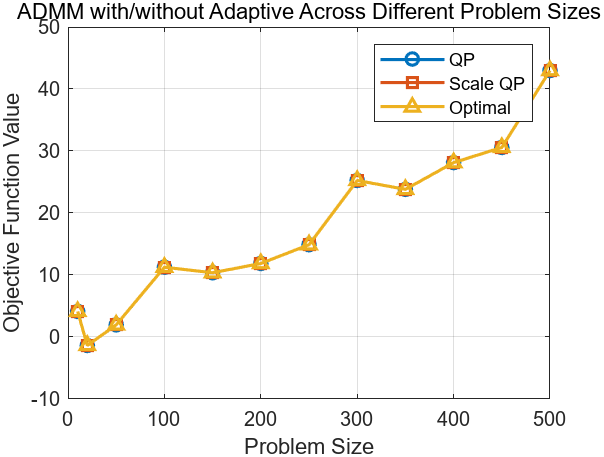
\includegraphics[width=0.75\linewidth]{fig/ADMM_Adaptive_rho.png}
    \caption{}
    \label{fig:Adaptive}
\end{figure}
\begin{figure}[H]
    \centering
    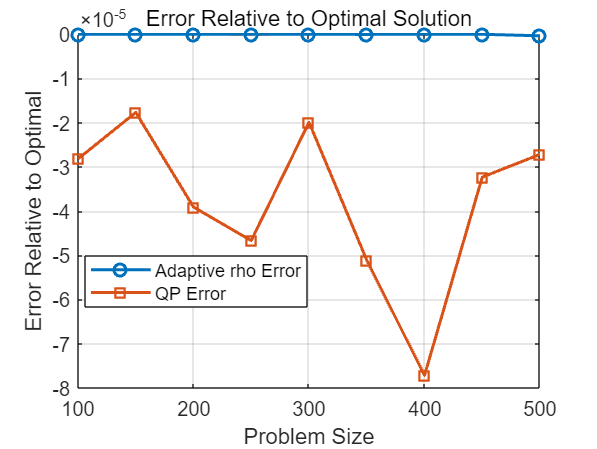
\includegraphics[width=0.75\linewidth]{fig/ADMM_Adaptive_rho_Error.png}
    \caption{Error Relative to Optimal Solution Using Adaptive Rho}
    \label{fig:Adaptive_Error}
\end{figure}

Figure~\ref{fig:Adaptive_Error} demonstrates the error relative to the optimal solution. The adaptive method could reduce the error compared to the standard fixed penalty approach, showcasing its effectiveness in improving accuracy and stability.



% \subsection{Additional Scenario Analysis}
% \subsubsection{Infeasible}
% Infeasibility arises when a quadratic programming (QP) problem's constraints cannot be satisfied simultaneously. This situation typically occurs due to inconsistencies in the equality or inequality constraints. Identifying infeasible problems is crucial, as attempting to solve them with iterative methods can lead to divergence or undefined behavior.

% To detect infeasibility, we employ the following conditions based on primal and dual residual checks:
% \begin{itemize}
%     \item \textbf{Primal Infeasibility:} 
%     If there exists a vector $\delta_y$ such that:
%     \[
%     \|\mathbf{A}^T \delta_y \|_\infty < \epsilon_{\text{prim\_inf}} \|\delta_y\|_\infty, \quad \text{and} \quad \mathbf{u}^\top \max(\delta_y, 0) + \mathbf{l}^\top \min(\delta_y, 0) < 0,
%     \]
%     then the problem is identified as primal infeasible.
%     \item \textbf{Dual Infeasibility:}
%     If there exists a vector $\delta_x$ satisfying:
%     \[
%     \mathbf{q}^\top \delta_x < 0, \quad \|\mathbf{P} \delta_x \|_\infty < \epsilon_{\text{dual\_inf}} \|\delta_x\|_\infty, \quad \text{and} \quad \mathbf{A} \delta_x \in \text{recession cone of } \mathbf{C},
%     \]
%     then the problem is identified as dual infeasible.
% \end{itemize}

% Detecting infeasibility early ensures that unnecessary computation is avoided, and infeasible certificates provide meaningful insights into constraint violations.

% \subsubsection{Non-convex}
% Non-convexity in quadratic programming occurs when the objective function $\phi(\mathbf{x}) = \frac{1}{2}\mathbf{x}^\top \mathbf{P} \mathbf{x} + \mathbf{q}^\top \mathbf{x}$ has a matrix $\mathbf{P}$ with negative eigenvalues, leading to local minima. Non-convex problems pose significant challenges as global optimization cannot be guaranteed using standard convex solvers.

% To identify non-convexity, we monitor the behavior of residuals:
% \begin{itemize}
%     \item Diverging residuals or unstable behavior during iterations may indicate that the problem is non-convex.
%     \item If the eigenvalues of $\mathbf{P}$ are computed and any are negative, the problem is classified as non-convex.
% \end{itemize}

% In our implementation, non-convex problems are flagged using termination checks on residuals. Specifically, if:
% \[
% \|\mathbf{P} \mathbf{x} + \mathbf{q} + \mathbf{A}^\top \mathbf{y}\|_\infty > \text{threshold},
% \]
% the solver assumes non-convexity and halts further iterations.

% Addressing non-convexity often requires specialized algorithms, such as global optimization or decomposition methods, which are outside the scope of standard QP solvers.

% \subsubsection{Degenerate}
% Degenerate may occur when the problem involves rank-deficient or ill-conditioned matrices. Under this condition, the degenerate system may get infinity solution. For example, in quadratic programming, if the matrix $\textbf{H}_{\text{tilde}}$ is not positive definite or has dependent rows, the optimization problem may become degenerate.

% To address this issue, we use \texttt{lsqminnorm} function in matlab. The \texttt{lsqminnorm} function computes the least-norm solution by leveraging the Moore-Penrose pseudoinverse: \[ \textbf{x}_{\text{next}} = \arg\min_{\textbf{x}} \quad \frac{1}{2} \textbf{x}^\top \textbf{H}_{\text{tilde}} \textbf{x} + \textbf{g}_{\text{tilde}}^\top \textbf{x}, \] where the matrix $\textbf{H}_{\text{tilde}}$ may be rank-deficient.

% This approach guarantees numerical stability and provides a well-defined solution even under degenerate conditions. By minimizing the Euclidean norm of the solution, \texttt{lsqminnorm} effectively avoids overfitting to any specific subset of constraints, ensuring that the resulting solution is optimal within the feasible region.

% Degenerate systems often arise in applications where constraints are inconsistent or redundant, making \texttt{lsqminnorm} a valuable tool for solving such problems robustly.


\section{Test and Evaluation}
\subsection{Experimental Design}

To evaluate the performance of the IRWA and ADMM algorithms, we designed an experimental setup involving the generation of Quadratic Programming (QP) problems. These problems require the matrix \(H\) to be positive semi-definite for convex optimization. We generated \(H\) by creating a random symmetric matrix and ensuring its positive definiteness through the addition of an identity matrix scaled by a positive constant. This process is mathematically described as:
\[
H = H_{\text{random}} + \alpha I_n,
\]
where \(H_{\text{random}}\) is a randomly generated symmetric matrix, \(I_n\) represents the identity matrix of size \(n \times n\), and \(\alpha > 0\) ensures all eigenvalues of \(H\) are non-negative, satisfying the convexity condition. This approach ensures that the resulting QP problems are well-posed and suitable for evaluating the performance of optimization algorithms.

The generated QP problems were solved using both the IRWA and ADMM algorithms. The performance of these algorithms was evaluated based on three primary metrics:
\begin{enumerate}
    \item \textbf{Number of Iterations}: Measures the convergence speed of the algorithm.
    \item \textbf{Constrained Residual and Duality Gap}: Quantifies the accuracy and feasibility of the solution.
    \item \textbf{Computation Time}: Captures the efficiency of the algorithm in solving QP problems of varying sizes.
\end{enumerate}

\subsubsection{First Experiment}

In the first experiment, we randomly generated 500 QP problems with different dimensions of the constraint matrix \(A\), specifically:
\[
A \in \mathbb{R}^{8 \times 20}, \quad A \in \mathbb{R}^{100 \times 200}, \quad A \in \mathbb{R}^{200 \times 500}.
\]
These dimensions were chosen to test the scalability and performance of the algorithms under a variety of problem sizes. For each iteration, we computed the percentage of solved problems to evaluate the convergence behavior of IRWA and ADMM.

\begin{figure}[htbp]
    \centering
    \begin{minipage}{0.49\linewidth}
        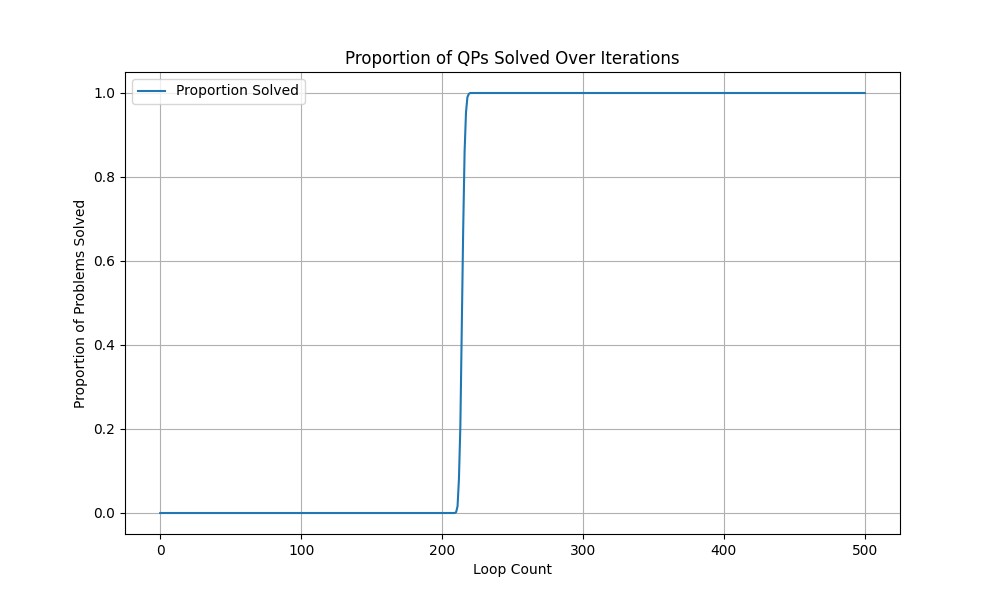
\includegraphics[width=\linewidth]{fig/IRWAQP_percentage_solved_LARGE.png}
        \caption{IRWA: Percentage of Problems Solved Over Iterations}
        \label{fig:IRWAQP_percentage_solved_LARGE}
    \end{minipage}
    \begin{minipage}{0.49\linewidth}
        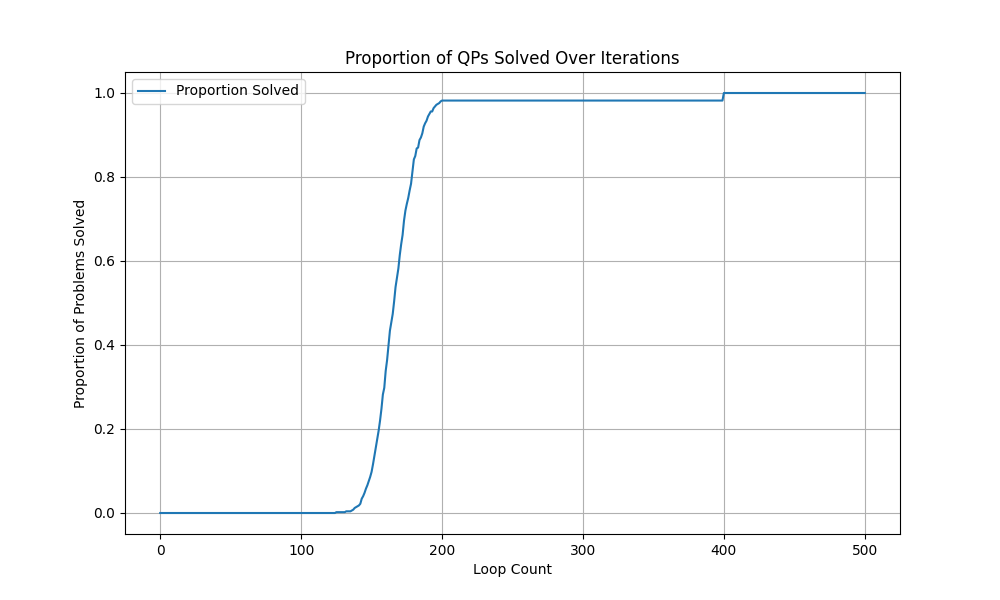
\includegraphics[width=\linewidth]{fig/ADMMQP_percentage_solved.png}
        \caption{ADMM: Percentage of Problems Solved Over Iterations}
        \label{fig:ADMMQP_percentage_solved_LARGE}
    \end{minipage}
\end{figure}

% The results of this experiment are illustrated in Figure~\ref{fig:IRWAQP_percentage_solved_LARGE} and Figure~\ref{fig:ADMMQP_percentage_solved_LARGE}. The distinct convergence behaviors of IRWA and ADMM are summarized as follows:
% \begin{itemize}
%     \item \textbf{IRWA:} In Figure~\ref{fig:IRWAQP_percentage_solved_LARGE}, we observe that the proportion of solved problems begins to increase significantly after approximately 200 iterations. This behavior suggests that IRWA requires additional iterations to refine its scaling adjustments and achieve feasibility. This delayed improvement indicates the computational overhead associated with IRWA's reweighting mechanism, which gradually resolves problem infeasibilities and achieves convergence.
    
%     \item \textbf{ADMM:} Figure~\ref{fig:ADMMQP_percentage_solved_LARGE} demonstrates that ADMM achieves rapid growth in the proportion of solved problems, starting at around 100 iterations. This earlier convergence highlights the inherent advantages of ADMM's distributed optimization approach, which efficiently handles constraints and accelerates the initial stages of progress. The faster convergence is particularly evident in smaller-sized problems.
% \end{itemize}
The experiment reveals key insights into the behavior of both algorithms. While ADMM demonstrates faster initial progress, IRWA eventually achieves comparable performance but requires more iterations to reach the same level of feasibility.

Figure~\ref{fig:IRWAQP_percentage_solved_LARGE} provides a clear view of IRWA’s gradual convergence process, where the percentage of solved problems remains minimal in the initial iterations but experiences a steep rise after approximately 200 iterations. In contrast,
Figure~\ref{fig:ADMMQP_percentage_solved_LARGE} underscores ADMM's ability to solve problems more quickly in the early stages. The rapid increase in the percentage of solved problems, beginning at around 100 iterations, showcases ADMM's effectiveness in leveraging distributed computation to address constraints and achieve feasibility efficiently.

In conclusion, these results underline the complementary strengths of IRWA and ADMM, with IRWA favoring accuracy and long-term stability and ADMM prioritizing speed and early feasibility. This experiment provides valuable guidance on selecting the appropriate algorithm for different problem scenarios.

\subsubsection{Second Experiment}
In this experiment, we compare the performance of IRWA and ADMM against the optimal solution of OSQP. The objective is to measure the relative deviation of the objective function values obtained by IRWA and ADMM from the optimal solution, as well as the differences between normal and accelerated IRWA methods. 

The results are calculated as the relative differences in the objective function values. It is represented as:
\[
\frac{\text{optimal value} - \text{optimal value of OSQP}}{\text{optimal value of OSQP}} \times 100
\]
This allows us to evaluate the effectiveness of acceleration techniques in improving the performance of IRWA. Additionally, the deviations of both IRWA and ADMM from OSQP's optimal solution provide insights into the trade-offs between different methods in terms of solution accuracy.


\begin{figure}[H]
    \centering
    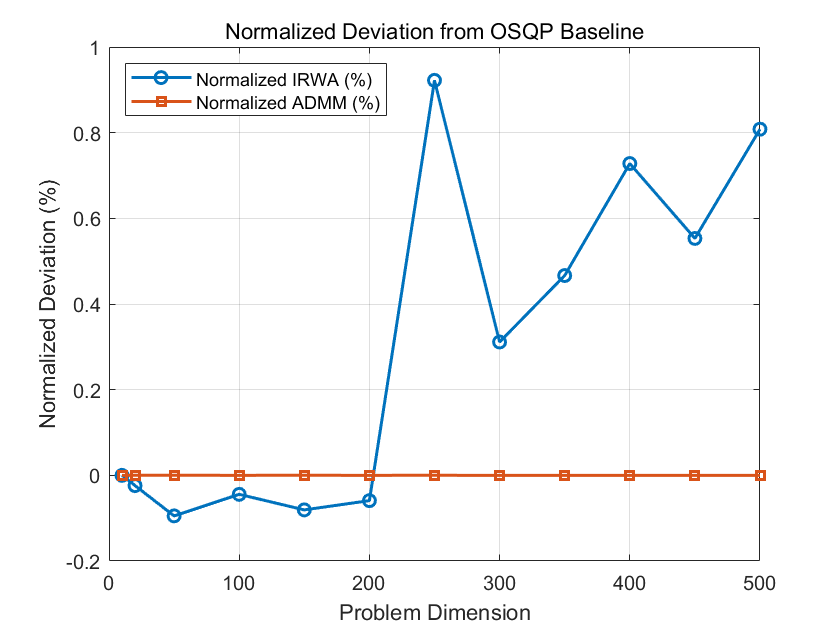
\includegraphics[width=0.75\linewidth]{fig/ADMM_vs_IRWA_of_optimal_value.png}
    \caption{}
    \label{fig:ADMM_vs_IRWA_normalized_deviation}
\end{figure}

The Figure \ref{fig:ADMM_vs_IRWA_normalized_deviation} shows that IRWA method exhibits larger fluctuations in normalized deviation compared to ADMM. While ADMM consistently maintains a normalized deviation close to 0\%, demonstrating its robustness and stability across all problem dimensions.

\subsubsection{Third Experiment}

This experiment evaluates the computation time of IRWA, ADMM, and OSQP (baseline) for problem sizes ranging from 20 to 500 dimensions. The average computation time is computed over 50 runs for each size. Figure~\ref{fig:Computation_time} shows the computation time for IRWA and ADMM, while Figure~\ref{fig:Computation_time_baseline} compares their runtime ratios relative to OSQP.

\begin{figure}[H]
    \centering
    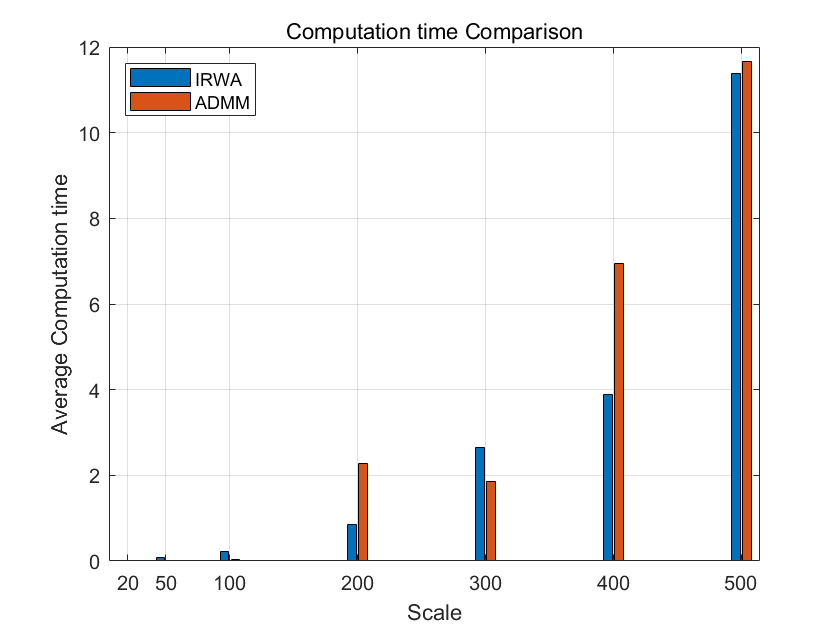
\includegraphics[width=0.75\linewidth]{fig/Computation_time.png}
    \caption{Computation time across different problem sizes for IRWA and ADMM}
    \label{fig:Computation_time}
\end{figure}

\begin{figure}[H]
    \centering
    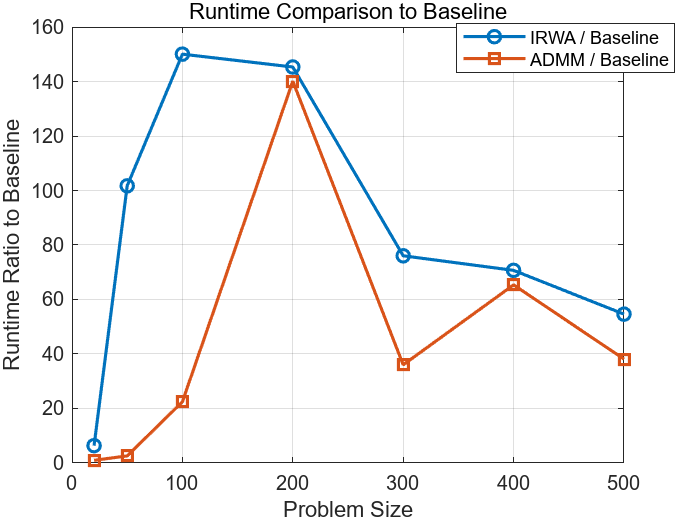
\includegraphics[width=0.75\linewidth]{fig/Computation_time_baseline.png}
    \caption{Comparison of runtime ratio to baseline (OSQP) for IRWA and ADMM}
    \label{fig:Computation_time_baseline}
\end{figure}

\paragraph{Analysis of Results}

\begin{itemize}
    \item \textbf{Computation Time Trends}:
    As shown in Figure~\ref{fig:Computation_time}, ADMM consistently achieves faster computation times than IRWA, particularly for medium-sized problems (200–300 dimensions). However, IRWA demonstrates more stable performance as problem sizes grow, albeit with a higher computation time overall.

    \item \textbf{Runtime Ratio to Baseline}:
    Figure~\ref{fig:Computation_time_baseline} illustrates the runtime ratio relative to OSQP. IRWA exhibits a sharp peak for problem sizes around 200, indicating increased overhead during scaling adjustments. ADMM maintains a lower runtime ratio but shows instability for medium-sized problems, potentially due to convergence challenges.

    \item \textbf{Large-Scale Performance}:
    For large problem sizes (above 400 dimensions), both IRWA and ADMM show improved relative efficiency, converging closer to the OSQP baseline, indicating better scalability for high-dimensional problems.
\end{itemize}

\paragraph{Conclusions}

ADMM demonstrates better overall efficiency and is well-suited for small to medium-sized problems. However, its performance instability for certain scales highlights the need for further optimization. IRWA, while slower, provides stable and reliable performance, making it more suitable for scenarios requiring robustness in handling complex constraints.


\bibliography{neurips_2024.bib}
\bibliographystyle{plain}
%%%%%%%%%%%%%%%%%%%%%%%%%%%%%%%%%%%%%%%%%%%%%%%%%%%%%%%%%%%%

\appendix

\section{Appendix / supplemental material}
\begin{itemize}
    \item Wiki: Quadratic programming. \\
    Available at: \url{https://en.wikipedia.org/wiki/Quadratic_programming}
    \item PyPI: qpsolvers\_benchmark. Benchmark for quadratic programming solvers available in Python. \\Available at: \url{https://pypi.org/project/qpsolvers_benchmark/} (accessed on December 12, 2024)
    \item GitHub: maros\_meszaros\_qpbenchmark. Benchmark datasets and test results for QP solvers. \\Available at: \url{https://github.com/qpsolvers/maros_meszaros_qpbenchmark} (accessed on December 12, 2024).
    \item Burke, J. V., Curtis, F. E., Wang, H., and Wang, J. (2015). Iterative Reweighted Linear Least Squares for Exact Penalty Subproblems on Product Sets. SIAM Journal on Optimization, 25(1), 261–294.\\
    Available at: \url{https://www.siam.org/journals/siopt/25-1/95023.html}
    % \item Stellato, B., Banjac, G., Goulart, P., Bemporad, A., \& Boyd, S. (2020). OSQP: An Operator Splitting Solver for Quadratic Programs. Mathematical Programming Computation, 12, 637–672. \\
    % DOI: \url{https://doi.org/10.1007/s12532-020-00179-2}.
\end{itemize}


\end{document}